\documentclass[10pt]{beamer}
%\usepackage[utf8]{inputenc}

\usetheme[progressbar=frametitle]{metropolis}
\usepackage{appendixnumberbeamer}

\usepackage{booktabs}
\usepackage[scale=2]{ccicons}

\usepackage{amsmath, amssymb, amsfonts}

\usepackage{pgfplots}
\usepgfplotslibrary{dateplot}

\usepackage{xspace}
\newcommand{\themename}{\textbf{\textsc{metropolis}}\xspace}

\usepackage[sfdefault, lining]{FiraSans}
\renewcommand*\oldstylenums[1]{{\firaoldstyle #1}}
\usepackage{newtxsf}
\usepackage{microtype}

\newcommand{\R}[0]{\mathbb{R}}
\newcommand{\bp}[0]{\mathbf{p}}
\newcommand{\bv}[0]{\mathbf{v}}
\newcommand{\bF}[0]{\mathbf{F}}
\DeclareMathOperator{\sign}{sign}

\title{Differenciálegyenletek}
\subtitle{Modellezés differenciálegyenletekkel}
% \date{\today}
\date{}
\author{Csikja Rudolf}
\institute{Budapesti Műszaki és Gazdaságtudományi Egyetem\\Matemaikai Intézet, Analízis Tanszék}
% \titlegraphic{\hfill\includegraphics[height=1.5cm]{logo.pdf}}

\begin{document}

\maketitle

%\begin{frame}{Table of contents}
%  \setbeamertemplate{section in toc}[sections numbered]
%  \tableofcontents%[hideallsubsections]
%\end{frame}


\section{Klasszikus mechanika}
\begin{frame}[t]{Newton-féle mozgásegyenlet}
Newton II. törvénye szerint egy test $\bp=m\bv$ lendületének (időbeli) megváltozása
arányos a testre ható erővel $\bp'(t) = \bF(t).$
A sebességre vonatkozó differenciálegyenlet így
\[\bv'(t) = \frac{1}{m}\bF(t)\]
\end{frame}

\begin{frame}[t]{Szabadesés}
\[
\begin{split}
v'(t)   &= \frac{1}{m}F_g = g
\end{split}
\]
hence
\[v(t) = v(0) + g t\]
Másfél perces esés végére a sebesség meghaladná a $3000\,$km/h-t.
\end{frame}

\begin{frame}[t]{Szabadesés légellenállással}
\begin{columns}
\column{0.5\textwidth}
    \[
    v'(t) = -\frac{1}{m}F_g + \frac{1}{m}F_D(v(t))
    \]
    a légellenállásból származó erő
    \[
    F_D(v) = -\frac{1}{2}\rho C_D A v^2 \sign(v)
    \]
    \begin{center}
    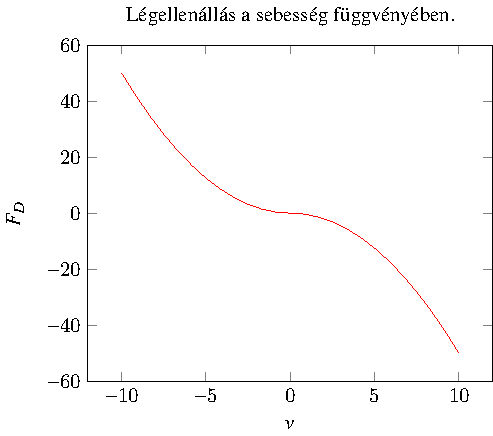
\includegraphics[width=0.8\textwidth]{drag_force.pdf}
    \end{center}
    \[v'(t) = -g + \frac{\rho C_D A}{2m} v^2(t), \quad v(t)\le 0.\]
\column{0.5\textwidth}
    \[v'(t) = -g\left(1-\left(\frac{v(t)}{V_T}\right)^2\right)\]
    A végsebesség feltétele $v'(t) = 0,$ amiből $V_{T} = \pm\sqrt{\frac{2 g m}{\rho C_D A}}.$
    \begin{center}
        
\includegraphics[scale=0.05]{skydive.png}
    \end{center}
    Az eredeti egyenlet felírható így:
Megoldás:
\[v(t) = V_T \left(\frac{2}{ 1 + \frac{V_T - v_0}{V_T + v_0}e^{\frac{2g}{V_T}t }} - 1\right)\]
\end{columns}
\end{frame}



\end{document}
